\documentclass{examen}

\begin{document}
\modulo{Lenguajes de marcas y sistemas de gesti�n de informaci�n}
\pregunta{Dado el archivo XML que se puede encontrar al final usar XPath para recuperar lo que se pide a continuaci�n
\begin{itemize}
\item{Recuperar todos nombres de proveedor sin incluir la marca nombreprov (1p)}
\item{Recuperar todos los elementos ciudad, est�n donde est�n (1p)}
\item{Recuperar el peso de las partes p1, p4 y p6 (1.5p)}
\end{itemize}
}{3.5}

\pregunta{Dado el archivo XML que se puede encontrar al final crear un archivo XSLT que tome dicho XML y genere un HTML como el que se muestra. En �l hay una lista desordenada (ul) con los nombres y estados de los proveedores cuya ciudad sea Londres. Debajo hay una lista desordenada (li) con los nombres y ciudad de partes azules que pesen 13 o m�s.}{6.5}

\begin{figure}[h]
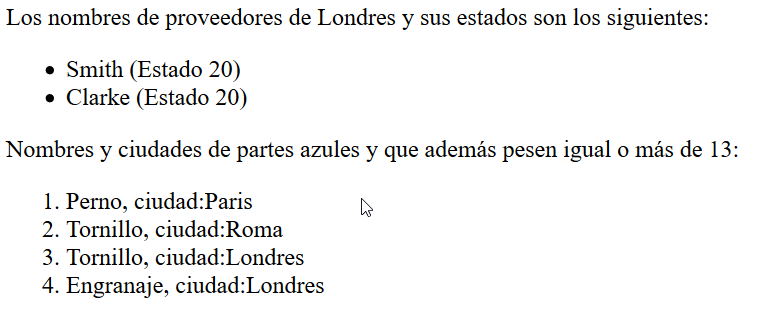
\includegraphics[scale=0.5]{captura.png}
\end{figure}
\begin{verbatim}
\end{verbatim}
\break
\begin{verbatim}
<datos>
    <proveedores>
        <proveedor numprov="v1">
            <nombreprov>Smith</nombreprov>
            <estado>20</estado>
            <ciudad>Londres</ciudad>
        </proveedor>
        ...Omitido...
    </proveedores>
    <partes>
        <parte numparte="p1">
            <nombreparte>Tuerca</nombreparte>
            <color>Rojo</color>
            <peso>12</peso>
            <ciudad>Londres</ciudad>
        </parte>
        ...Omitido...
    </partes>
    <proyectos>
        <proyecto numproyecto="y1">
            <nombreproyecto>Clasificador</nombreproyecto>
            <ciudad>Paris</ciudad>
        </proyecto>
        ...Omitido...
    </proyectos>
    <suministros>
        <suministra>
            <numprov>v1</numprov>
            <numparte>p1</numparte>
            <numproyecto>y1</numproyecto>
            <cantidad>200</cantidad>
        </suministra>
        ...Omitido...
    </suministros>
</datos>
\end{verbatim}
\end{document}
